% siminos/kittens/catHamilton.tex                   pdflatex CL18
% $Author: predrag $ $Date: 2020-07-28 01:02:24 -0500 (Tue, 28 Jul 2020) $

\section{Cat map: Hamiltonian formulation}
\label{s:catMapHam}
    % earlier names:
    % siminos/spatiotemp/chapter/catHamilton.tex
    % \section{Life of a single Hamiltonian cat}

\subsection{\AW\ partition of the cat map \statesp}
\label{s:catAW}

%%%%%%%%%%%%%%%%%%%%%%%%%%%%%%%%%%%%%%%%%%%%%%%%%%%%%%%%%%%%%
% PC 2018-02-09 PVAdlerWeissB-a.svg started from PCLect13p9.svg
% PC 2018-02-09 PVAdlerWeissB-b.svg started from PCLect13p15.svg
% PC 2018-02-09 PVAdlerWeissB-c.svg started from PCLect13p16a.svg
% PC 2018-02-09 PVAWMarkov.svg B&W started from Lect13p17.pdf
% PC 2018-02-11 PVAWMarkovCol.svg  started from PVAWMarkov.svg
%               bit too big - redraw from scratch
\begin{figure}\begin{center}
            \begin{minipage}[c]{0.23\textwidth}\begin{center}
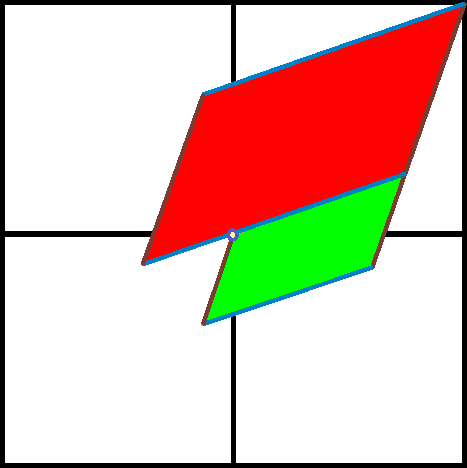
\includegraphics[width=1.0\textwidth]{PVAdlerWeissB-a}\\(a)
            \end{center}\end{minipage}
            \begin{minipage}[c]{0.23\textwidth}\begin{center}
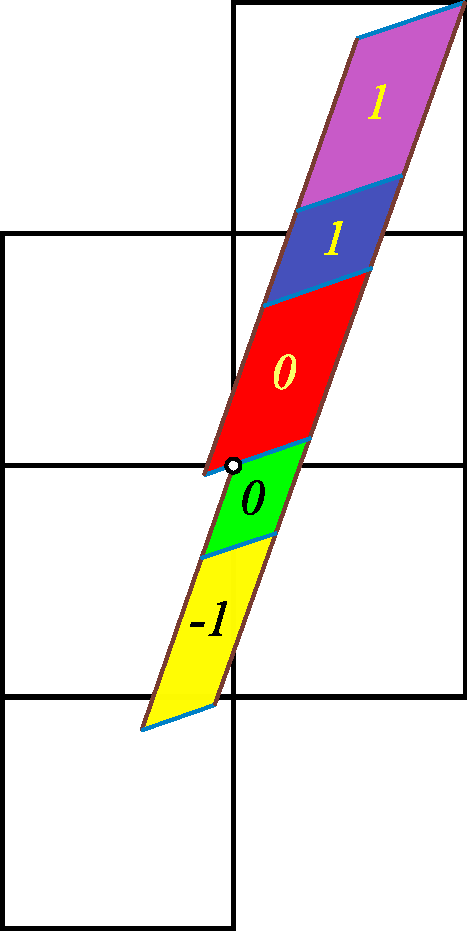
\includegraphics[width=1.0\textwidth]{PVAdlerWeissB-b}\\(b)
            \end{center}\end{minipage}
            \begin{minipage}[c]{0.23\textwidth}\begin{center}
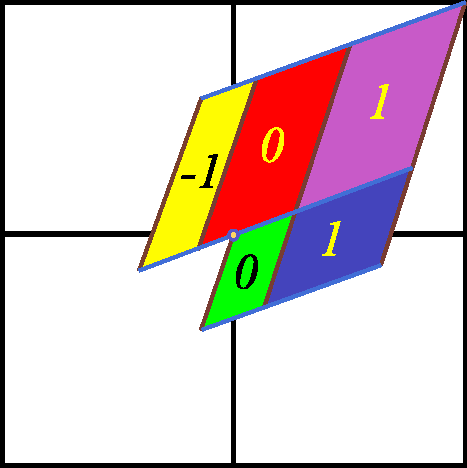
\includegraphics[width=1.0\textwidth]{PVAdlerWeissB-c}\\(c)
            \end{center}\end{minipage}
            ~~~
            \begin{minipage}[c]{0.12\textwidth}\begin{center}
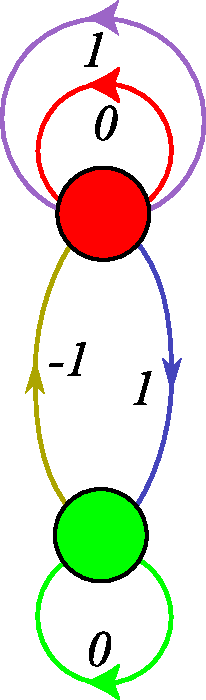
\includegraphics[width=1.0\textwidth]{PVAWMarkovCol}\\(d)
            \end{center}\end{minipage}
\end{center}
  \caption{\label{fig:PVAdlerWeiss}
(Color online)
(a)
An \AW\ generating partition of the unit torus for the $s=3$ \PV\ cat map
\refeq{eq:StateSpCatMap}, with rectangle $\pS_A$ (red) and $\pS_B$
(green) borders given by the cat map stable (blue) and unstable (dark
red) manifolds, \ie, along the two eigenvectors corresponding to the
eigenvalues \refeq{StabMtlpr}.
(b)
Mapped one step forward in time, the rectangles are stretched along the
unstable direction and shrunk along the stable direction. Sub-rectangles
$\pS_j$ that have to be translated back into the partition are indicated by
color and labeled by their lattice translation
$\Ssym{j}\in\A=\{\underline{1},0,1\}$, which also doubles as the 3-letter
alphabet $\A$.
(c)
The sub-rectangles $\pS_j$ translated back into the initial partition
yield a generating partition, with the finite grammar given by the
{\markGraph}
(d).
The nodes
refer to the rectangles $A$ and $B$, and the five links correspond to the five
sub-rectangles induced by one step forward-time dynamics.
For details, see ChaosBook\rf{DasBuch}.
% make ChaosBook link specific.
}
\end{figure}
%%%%%%%%%%%%%%%%%%%%%%%%%%%%%%%%%%%%%%%%%%%%%%%%%%%%%%%%%%%%%%%

Cat maps, also known as Thom-Anosov diffeomorphisms, or
Thom-Anosov-Arnol'd-Sinai {cat maps}\rf{ArnAve,deva87,StOtWt06}, have
been extensively studied as the simplest examples of chaotic Hamiltonian
systems.

\PV\ cat map \refeq{eq:StateSpCatMap} is a discrete time non-autonomous
Hamiltonian system, time-forced by `pulses' $\Ssym{\zeit}$.
The $\Ssym{\zeit}$ translations reshuffle the \statesp, as in
\reffig{fig:PVAdlerWeiss}, thus partitioning it into regions
$\pS_\Ssym{}$, labeled with letters $\Ssym{}$ of the $|\A|$-letter
alphabet $\A$, and associating a symbol sequence $\{\Ssym{\zeit}\}$ to
the dynamical trajectory $\{\ssp_{\zeit}\}$. As the relation
\refeq{eq:StateSpCatMap} between the trajectory \(\ssp_{\zeit}\) and its
symbolic dynamics encoding \(\m_{\zeit}\) is linear, Percival and Vivaldi
refer to \(\m_{\zeit}\) as a `linear code'.

As explained in the companion paper\rf{GHJSC16},
the deep problem with the \PV\ code prescription is that it does not
yield a generating partition; the borders (\ie, $\ssp_0$, $\ssp_1$ axes)
of their unit-square partition
$(\ssp_{\zeit-1},\ssp_{\zeit})\in(0,1]\times(0,1]$
do not map onto themselves, resulting in the infinity of, to us unknown,
grammar rules for {\inadmissible} symbol sequences.

This problem was resolved in 1967 by Adler and
Weiss\rf{AdWei67,ArnAve,AdWei70} who utilized the stable/\-unstable
manifolds of the fixed point at the origin to cover a unit area torus by
a two-rectangles generating partition; for the \PV\ cat map
\refeq{eq:StateSpCatMap}, such partition\rf{DasBuch} is drawn in
\reffig{fig:PVAdlerWeiss}. Following Bowen\rf{Bowen70}, one refers to
parallelograms in \reffig{fig:PVAdlerWeiss} as `rectangles'; for details
see Devaney\rf{deva87}, Robinson\rf{Robinson12}, or
ChaosBook\rf{DasBuch}. Siemaszko and Wojtkowski\rf{SieWoj11} refer to
such partitions as the `Berg partitions', and Creagh\rf{Creagh94} studies
their generalization to weakly nonlinear mappings. Symbolic dynamics on
this partition is a subshift of finite type, with the 3-letter alphabet
\beq
\A=\{\underline{1},0,1\}
\ee{catAlphabetPVAW}
that indicates the translation needed to return the given sub-rectangle
$\pS_{{j}}$ back into the two-rectangle partition $\pS= \pS_{{A}}\cup
\pS_{{B}}$.

While Percival and Vivaldi were well aware of \AW\ partitions, they felt
that their ``coding is less efficient in requiring more symbols, but it
has the advantage of linearity.'' Our construction demonstrates that one
can have both:  an \AW\ generating cat map partition, and a linear code.
The only difference from the \PV\ formulation\rf{PerViv} is that one
trades the single unit-square cover of the torus of
\refeq{eq:StateSpCatMap} for the dynamically intrinsic, two-rectangles
cover of \reffig{fig:PVAdlerWeiss}, but the effect is magic - now every
infinite walk on the {\markGraph}  of \reffig{fig:PVAdlerWeiss}\,(d)
corresponds to a unique {\admissible} orbit $\{\ssp_{\zeit}\}$, and the
{\markGraph} generates all {\admissible} itineraries $\{\Ssym{\zeit}\}$.

To summarize:
an explicit \AW\ generating partition, such as
\reffig{fig:PVAdlerWeiss}, completely solves the Hamiltonian cat map
problem, in the sense that it generates all {\admissible} orbits.
Rational and irrational initial states generate periodic and ergodic
orbits, respectively\rf{PerViv87b,Keating91}, with every \statesp\ orbit
uniquely labeled by an {\admissible} bi-infinite itinerary of symbols
from alphabet \A.

\subsection{Counting Hamiltonian cat map \po s}
\label{s:catHamCount}

                                \toCB
    %\PC{2019-08-01}{
The five sub-rectangles $\pS_{{j}}$ of the two-rectangle \AW\ partition
of \reffig{fig:PVAdlerWeiss}\,(c) motivate introduction of a 5-letter
alphabet
\beq
\Aa=\{ {1}, {2}, {3}, {4}, {5}\}
  = \{A{}^0\!A, B{}^1\!A, A{}^1\!A, B{}^0\!B, A{}^{\underline{1}}\!B\}
\,,
\ee{cat5AlphabetPVAW}
see \reffig{fig:PVAdlerWeissS}\,(b), which encodes the links of the
{\markGraph}  of \reffig{fig:PVAdlerWeiss}\,(d). The loop expansion  of
the determinant\rf{CBcount} of the {\markGraph} $T$ of
\reffig{fig:PVAdlerWeissS}\,(b)  is given by all non-intersecting walks
on the graph
\beq
\det(1-zT) = 1 - z(t_1+t_3+t_4)
               - z^2 (t_{25}-(t_1+t_3)t_4)
 \,,
\ee{CatMapDetTransMat}
where $t_p$ are traces over fundamental cycles, the three fixed points
\(
t_1 = T_{A{}^0\!A},
t_3 = T_{A{}^1\!A},
t_4 = T_{B{}^0\!B},
\)
and the 2-cycle
\(
t_{25} = T_{B{}^{1}\!A} T_{A{}^{\underline{1}}\!B}
\,.
\)

As the simplest application, consider counting all {\admissible} cat map
\po s. This is accomplished  by setting the non-vanishing links of the
{\markGraph} to $T_{ji}=1$, resulting in the ${s}=3$ cat map
\tzeta\rf{Isola90,DasBuch},
\beq
\zetatop(z) =  \frac{1 - 3 z + z^2}
                  {(1 - z)^2}
\,,
\ee{Isola90-13a}
where the numerator ${(1 - z)^2}$ corrects the overcounting of the fixed
point at the origin due to assigning it to both $\pS_A$ (twice) and
$\pS_B$ rectangles\rf{manning}.

    \PC{2020-02-08}{
Note:
$N_2=\Det\jMorb=({s}-2)({s}+2)$,
$N_3 %   = {s}^3-3{s}-2
    = ({s}-2)({s}+1)^2$,
$N_4 = ({s}-2)({s}+1)\,{s}^2$,
$N_5 = ({s}-2)(s^2+ s-1 )^2$.
I think the factorization is true for all $\cl{}$, as the $s=2$ Laplacian
has a zero mode (constant $\ssp_i$, I think).

an sequence of non-negative integers counting the orbits of
a map; the sequence of periodic points for that map.
    }


%    \PCpost{2020-01-16}
                               \toCB
The number of \emph{periodic points} of
period $n$ is given by \refeq{zetatop-N}, the logarithmic derivative of
the {\tzeta}. Substituting the cat map \tzeta\ \refeq{Isola90-13a} we
obtain
% ------------------- siminos/mathematica/ ----------
% CatMaptopZeta.nb                                    2020-01-16
%    Cat map periodic points counting for CL18.tex
% 1,5,16,45,121,320,841,2205,5776,15125,39601,
\bea
\sum_{n=1}N_n z^n
    &=&
 z+5 z^2+16 z^3+45 z^4+121 z^5+320 z^6+841 z^7
    \ceq
+2205 z^8+5776 z^9+15125 z^{10}
+39601 z^{11}
+\cdots
%+O\left(z^{11}\right)
\label{catMapN_n-s=3}
\eea
WolframAlpha says, compare with \refeq{1stChebGenF}:
\beq
\sum_{n=1}N_n z^n % = \frac{-z - 1}{z^3 - 4 z^2 + 4 z - 1}
            % = \frac{-z - 1}{(z - 1) (z^2 - 3 z + 1)}
            = \frac{s - 2 z}{1 - s z + z^2} - \frac{2}{1 - z}
\ee{s=3PPs}

The number of \emph{prime} cycles is given by
\refeq{primeCount},
% ------------------- siminos/mathematica/ ----------
% CatMaptopZeta.nb                                    2020-01-16
%    Cat map periodic points counting for CL18.tex
% 1,2,5,10,24,50,120,270,640,1500,3600,...
% see https://oeis.org/A032170 https://oeis.org/A072337
%     https://oeis.org/A004146/internal
% a(n) = 2*(T(n, 3/2)-1)with Chebyshev's polynomials T(n, x) of the first kind.
%        See their coefficient triangle https://oeis.org/A053120
% a(n) = 2*T(n, 3/2) - 2, with twice the Chebyshev's polynomials of the first kind,
%                           2*T(n, x=3/2)= https://oeis.org/A005248
\bea
\sum_{n=1}M_n z^n
    &=&
 z+2 z^2+5 z^3+10 z^4+24 z^5+50 z^6+120 z^7
    \ceq
+270 z^8+640 z^9+ 1500z^{10}+3600 z^{11}
+\cdots
% +O\left(z^{11}\right)
\,,
\label{catMapM_n-s=3}
\eea
in agreement with the Bird and Vivaldi\rf{BirViv} census.
% (they call that $N_T(\lambda)$ in their Table~1, with $s=K=3$ and $4$),

%%%%%%%%%%%%%%%%%%%%%%%%%%%%%%%%%%%%%%%%%%%%%%%%%%%%%%%%%%%%%
\begin{figure}\begin{center}
            \begin{minipage}[c]{0.30\textwidth}\begin{center}
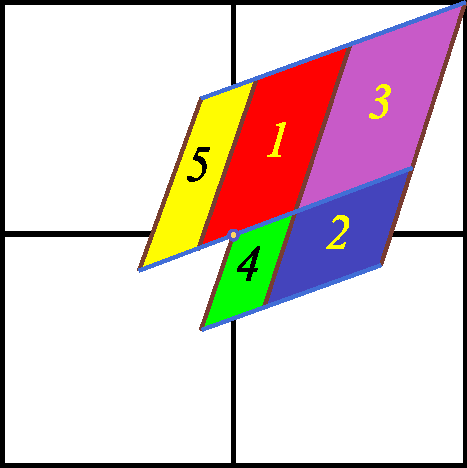
\includegraphics[width=1.0\textwidth]{PVAdlerWeissS-c}\\(a)
            \end{center}\end{minipage}
            \hskip 8ex
            \begin{minipage}[c]{0.12\textwidth}\begin{center}
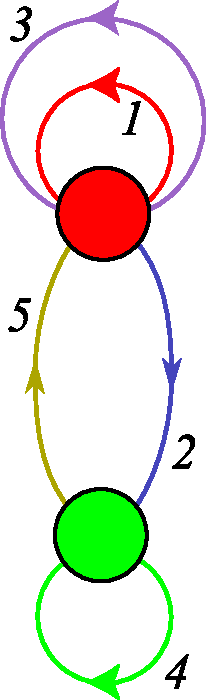
\includegraphics[width=1.0\textwidth]{PVAWMarkovSymb}\\(b)
            \end{center}\end{minipage}
\end{center}
  \caption{\label{fig:PVAdlerWeissS}
(Color online)
(a)
The sub-rectangles $\pS_j$ of \reffig{fig:PVAdlerWeiss}\,(c).
(b)
Admissible orbits correspond to walks on the {\markGraph} of
\reffig{fig:PVAdlerWeiss}\,(d), with rectangles $\pS_A$ (red) and
$\pS_B$ (green) as nodes, and the links labeled by
5-letter alphabet \refeq{cat5AlphabetPVAW}, see the
loop expansion \refeq{CatMapDetTransMat}.
}
\end{figure}
%%%%%%%%%%%%%%%%%%%%%%%%%%%%%%%%%%%%%%%%%%%%%%%%%%%%%%%%%%%%%%%

%%%%%%%%%%%%%%%%%%%%%%%%%%%%%%%%%%%%%%%%%%%%%%%%%%%%%%%%%%%%%%%
\begin{figure}
  \centering
(a)   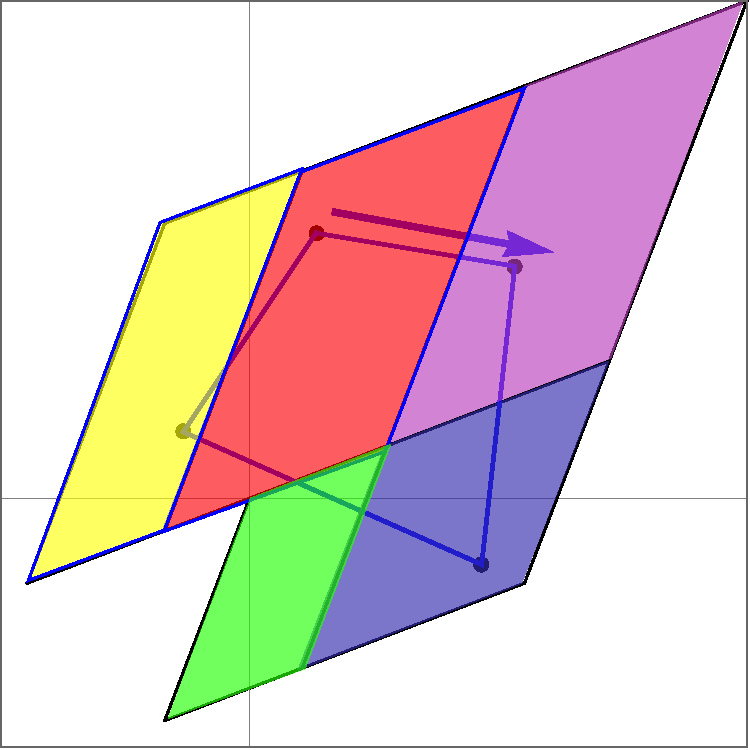
\includegraphics[width=0.35\textwidth]{HLPeriodicOrbit5}
\hskip 1ex
(b)   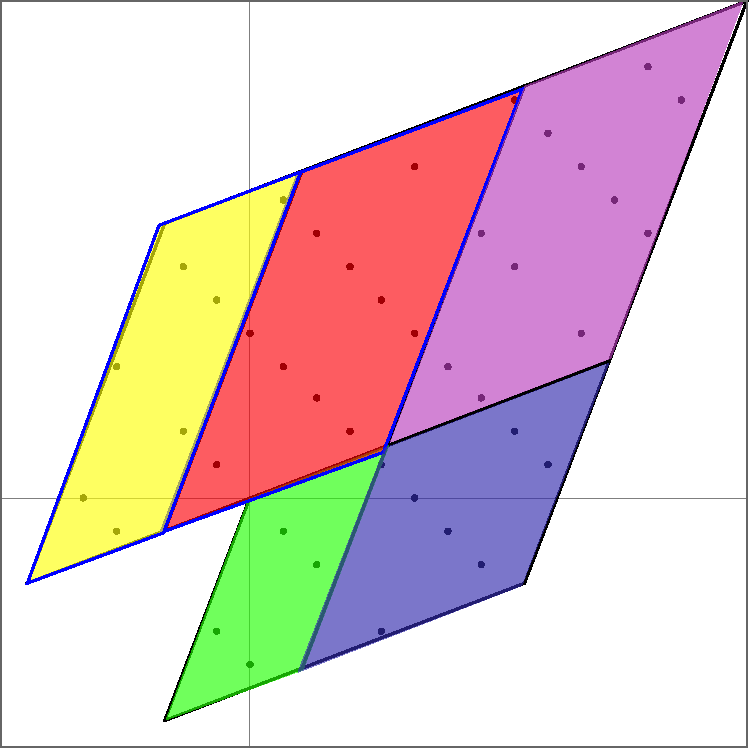
\includegraphics[width=0.35\textwidth]{HLAllCyclePointsB}
      % from \reffig{fig:HLAllCyclePoints}
 	\caption{\label{fig:HLPeriodicOrbitsA}
(a) An example of a 4-cycle:
$\Xx_{0 1 1 \underline{1}}$. %\frac{1}{15}(2,8,7,-2)$,
(b) All prime period-4 lattice states land in the partition of
\reffig{fig:PVAdlerWeissS}\,(a).
% Added colors to these two figures so readers can compare the orbit
% with the transition graph \reffig{fig:PVAdlerWeissS} (b).
}
\end{figure}
%%%%%%%%%%%%%%%%%%%%%%%%%%%%%%%%%%%%%%%%%%%%%%%%%%%%%%%%%%%%%%%

This derivation was based on the \AW\ generating partition, a clever
explicit visualization of the cat map dynamics, whose generalization to
several coupled maps (let alone spatially infinite coupled cat
maps lattice) is far from obvious: one would have to construct covers of
high-dimensional {\fundPip}s by sets of sub-volumes.
However, as Keating\rf{Keating91} explains, no such explicit generating
partition is needed to count cat map \po s.
Cat map \refeq{eq:StateSpCatMap} lattice states are the fixed points of
\[
\left[\begin{array}{c}
  \coord_\zeit  \\ p_\zeit
  \end{array}\right]
=
   \left[\begin{array}{c}
  \coord_{\zeit+\cl{}}  \\ p_{\zeit+\cl{}}
  \end{array}\right]
=
  \jMps^\cl{}
  \left[\begin{array}{c}
  \coord_\zeit  \\ p_\zeit
  \end{array}\right]
  \quad (\mbox{mod}\;1)
\,,
\]
so on the unwrapped phase space lattice, tiled by repeats of the
unit square of the cat map torus,
\beq
 (\jMps^\cl{} - \matId)
    \left[\begin{array}{c}
 \coord_\zeit  \\ p_\zeit
    \end{array}\right]
=
    \left[\begin{array}{c}
m_{\zeit}^\coord \\ m_{\zeit}^p
    \end{array}\right]
\,,\qquad
    (m_{\zeit}^\coord,m_{\zeit}^p)\in\integers^2
\,,
\ee{fundParallelo}
matrix $(\jMps^\cl{} - \matId)$ stretches the unit square into
the `{\fundPip}'.

\subsection{An example: period-4 prime cycles}
\label{s:cat4cycles}

% \PCpost{2018-02-11}{
As a hands-on example, let us count the $M_4=10$ {\admissible} prime
4-cycles, as stated in \refeq{noPrimeCycs=3}.
The {\admissible} \brick s $\Mm_p$ can be read off as walks on
either the 5-letter alphabet \refeq{cat5AlphabetPVAW} graph, see
\reffig{fig:PVAdlerWeissS}\,(b),
or the 3-letter alphabet \refeq{catAlphabetPVAW} graph, see
\reffig{fig:PVAdlerWeiss}\,(d). They are, in 5-letter (top), and
3-letter (bottom) alphabets
        \PC{2019-12-20}{
For covering symbolic dynamics, use/refer to ChaosBook.

Order \refeq{prime4cycles} lexically.
    }

\bea
&&
\begin{array}{c} \cycle{1113} \\  0 0 0            1 \end{array} \;
\begin{array}{c} \cycle{1125} \\  0 0 1 \underline{1}\end{array} \;
\begin{array}{c} \cycle{1245} \\  0 1 0 \underline{1}\end{array} \;
\begin{array}{c} \cycle{1253} \\  0 1 \underline{1}1 \end{array} \;
\begin{array}{c} \cycle{1325} \\  0 1 1 \underline{1}\end{array} \;
        \continue
&&
\begin{array}{c} \cycle{1133} \\  0 0 1            1 \end{array} \;
\begin{array}{c} \cycle{3325} \\  1 1 1 \underline{1}\end{array} \;
\begin{array}{c} \cycle{3331} \\  1 1 1            0 \end{array} \;
\begin{array}{c} \cycle{3245} \\  1 1 0 \underline{1}\end{array} \;
\begin{array}{c} \cycle{4452} \\  0 0 \underline{1}1 \end{array}
\,.
\label{prime4cycles}
\eea
% with the corresponding overall translation per cycle given by
% the sum of the 3-letter alphabet labels.

% \HLpost{2018-02-11}{
The corresponding \po s $\Xx_p$ are computed using Green's function
\refeq{1dLatGreenFct} (the inverse of the $[4\times4]$ {\jacobianOrb} \refeq{Hessian},
easiest to evaluate by discrete Fourier transforms, see
\refappe{appe:Fourier}):
\[
\Mm_{0 0 0 1}
            \Rightarrow\quad
\Xx_{0 0 0 1}= g
\left[\begin{array}{c}
 0 \\
 0 \\
 0 \\
 1 \\
\end{array}\right]
   =
\frac{1}{15}
\left[\begin{array}{c}
 {3} \\
 {2} \\
 {3} \\
 {7} \\
\end{array}\right]
\,.
\]
Likewise,
        \PC{2019-12-20}{
To Han: order lexically.
    }

\bea
\transp{\Xx}_{0 0 1 \underline{1}} &=& \frac{1}{15}
\left[\begin{array}{cccc}
 {-1} &
 {1} &
 {4} &
 {-4}
\end{array}\right]
    \,,\qquad
\transp{\Xx}_{0 1 0 \underline{1}}= \frac{1}{15}
\left[\begin{array}{cccc}
 {0} &
 {5} &
 {0} &
 {-5}
\end{array}\right]
    \continue
\transp{\Xx}_{0 1 \underline{1}1} &=& \frac{1}{15}
\left[\begin{array}{cccc}
 {4} &
 {6} &
 {-1} &
 {6}
\end{array}\right]
    \,,\qquad~~
\transp{\Xx}_{0 1 1 \underline{1}}= \frac{1}{15}
\left[\begin{array}{cccc}
 {2} &
 {8} &
 {7} &
 {-2}
\end{array}\right]
    \continue
\transp{\Xx}_{0 0 1 1} &=& \frac{1}{15}
\left[\begin{array}{cccc}
 {5} &
 {5} &
 {10} &
 {10}
\end{array}\right]
    \,,\qquad~~
\transp{\Xx}_{1 1 1 \underline{1}}= \frac{1}{15}
\left[\begin{array}{cccc}
 {9} &
 {11} &
 {9} &
 {1}
\end{array}\right]
    \continue
\transp{\Xx}_{1 1 1 0} &=& \frac{1}{15}
\left[\begin{array}{cccc}
 {12} &
 {13} &
 {12} &
 {8}
\end{array}\right]
    \,,\qquad
\transp{\Xx}_{1 1 0 \underline{1}}= \frac{1}{15}
\left[\begin{array}{cccc}
 {7} &
 {8} &
 {2} &
 {-2}
\end{array}\right]
    \continue
\transp{\Xx}_{0 0 \underline{1}1} &=& \frac{1}{15}
\left[\begin{array}{cccc}
 {1} &
 {-1} &
 {-4} &
 {4}
\end{array}\right]
\,.
\label{4-cyclePPs}
\eea
One can verify that for each of these 10 prime 4-cycles the  lattice
states $(\ssp_t,\ssp_{t+1})$ visit the rectangles $\pS_A$ or $\pS_B$ of
\reffig{fig:PVAdlerWeiss}\,(b) in the temporal order dictated by the
\markGraph, and thus they are all {\admissible} cycles.
    \PC{2020-01-28}{
Perhaps summarize here our failed efforts to make an time-reversal
invariant \AW\ partition; Ihara zeta functions, ...
    }
